\documentclass[conference]{IEEEtran}
\IEEEoverridecommandlockouts
% The preceding line is only needed to identify funding in the first footnote. If that is unneeded, please comment it out.
\usepackage{cite}
\usepackage{amsmath,amssymb,amsfonts}
\usepackage{graphicx}
\usepackage{textcomp}
\usepackage{xcolor}
\def\BibTeX{{\rm B\kern-.05em{\sc i\kern-.025em b}\kern-.08em
    T\kern-.1667em\lower.7ex\hbox{E}\kern-.125emX}}
\title{
\vspace{1cm}
{
\includegraphics[width=0.15\textwidth]{iithlogo.jpg} \\ Platformio Assignment} }
\author{Akkugari Ruchika \\ Roll No: FWC22276 \\ akkugariruchika@gmail.com}
 \begin{document}
\maketitle
 \section {ABSTRACT}
 The sequence of states $(Q_{1}Q_{0})$ of the given synchronous sequential circuit is:
 \begin {figure}[h]
 \centering
 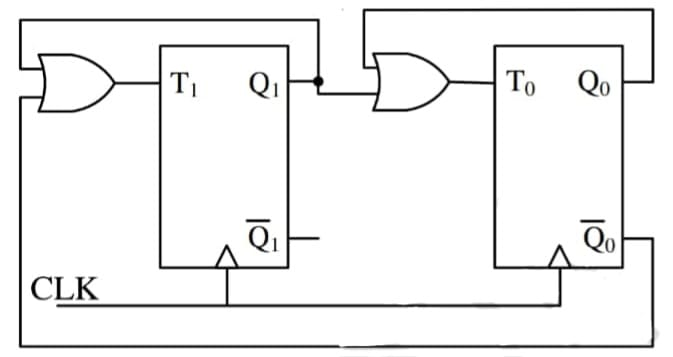
\includegraphics[width=0.35\textwidth]{pltio.jpg}
 \caption{\label{fig: Sequential Circuit}}
 \end {figure}
\section{COMPONENTS}
The required components list is given in Table: I. Flip-flop IC 7474 diagram is shown in Fig.2.
\begin{figure}[h]
\centering
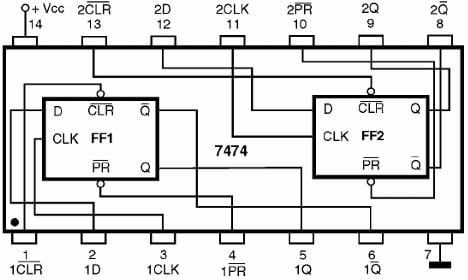
\includegraphics[width=0.35\textwidth]{7474ic.jpg}
\caption{\label{fig:Gates}}
\end{figure}
 \begin{table} [htbp]
\centering
\begin{tabular}{| c | c | c |} \hline
Components & Value & Quantity \\\hline
IC & 7474 & 1 \\ \hline
LEDs &  & 2 \\ \hline
Arduino & UNO & 1 \\ \hline
Jumper Wires &  & 20 \\ \hline
Breadboard & & 1 \\ 
\hline
\end{tabular}
\vspace{0.1cm}
\caption{\label{tab:widgets}}
\end{table}\\
\section{PROCEDURE}
By using 7474 IC we can implement T-flip flop. 7474 IC contains two D-flip flops. T-flip flop logic is implemented by using D-flip flop, this is done by giving XOR logic to the output of D flip flop. The XOR and OR gate logic is given in the arduino code. Make the connections between the arduino and the IC according to the given circuit. The truth table for the given circuit is:
 \begin{table}[htbp]
	 \centering
	 \begin{tabular}{| c | c | c |}\hline
		 CLK & $T_{1}T_{0}$ & $Q_{1}Q_{0}$\\
		 \hline
		  & & 00\\ \hline
		  & 10 & 10\\ \hline
		  & 11 & 01\\ \hline
		  & 01 & 00\\
		  \hline
	 \end{tabular}
	 \vspace{0.1cm}
	 \caption{\label{tab:widgets}}
 \end{table}
\section{RESULTS}
Download the code given in the link below and execute them to see the output as shown in Fig.3 by placing the LED at the output pin of 7474 IC, where the states of the sequential circuit are shown through the LED's : $00\rightarrow10\rightarrow01\rightarrow00$
https:
\begin{figure}[h] 
	\centering 
	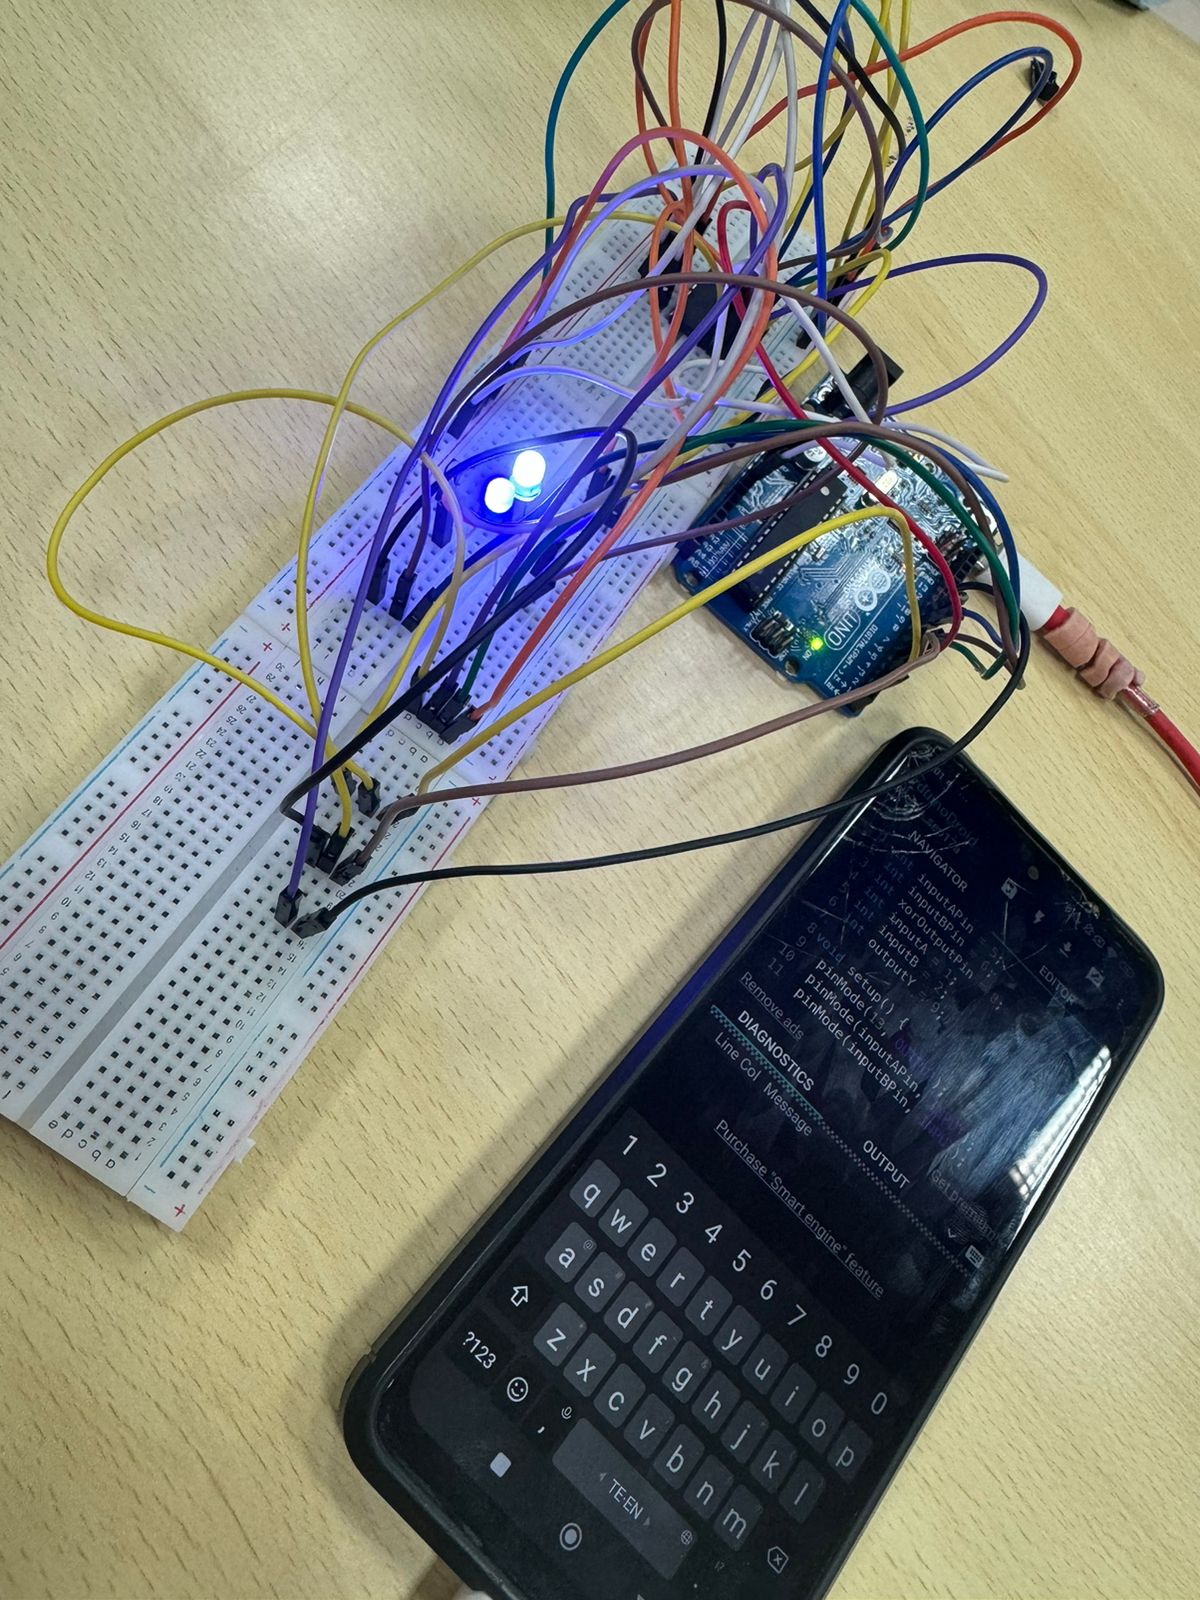
\includegraphics[width=0.4\textwidth]{img11.jpg}
	\caption{\label{fig:Result}}    
\end{figure}
\section{CONCLUSION}
In conclusion, the T flip-flop, known for toggling its output with each clock pulse when the input is high, can be effectively implemented using the 7474 IC, a D flip-flop. By incorporating an XOR gate, the 7474 IC's behaviour is modified to achieve the desired toggling charecteristic of the T flip-flop. This setup demonstrates the versatility of the 7474 IC and highlights how flip-flops can be adapted for different digital logic functions, making them essential components in sequential circuits and therefore, we can design several circuits and can be implemented using Arduino and Platformio.
\end{document}
